%%%%%%%%%%%%
%
% $Autor: Wings $
% $Datum: 2019-03-05 08:03:15Z $
% $Pfad: Automatisierung/Skript/Produktspezifikation/Powerpoint/AMF.tex $
% $Version: 4250 $
%
%%%%%%%%%%%%



%todo Eigene Bilder
%todo https://ieeexplore.ieee.org/abstract/document/8100841 lena   - general\

\section{Bilder und Bildklassifizierung mit einem \ac{cnn}}


Die Klassifikation von Bildern teilt sich in zwei Bereiche: der Bild- und der Objektklassifikation. 
Bei der Objektklassifikation wird versucht, ein oder mehrere Objekte zu identifizieren. Die Identifikation erfolgt durch eine Zuordnung zu vorgegebenen Klassen. In der Regel werden die Ergebnisse mit Wahrscheinlichkeiten angegeben. Bei der Bildklassifikation wird versucht, eine geeignete Beschreibung für das Bild zu ermitteln; in diesem Fall wird das Bild in seiner Gesamtheit erfasst und interpretiert. \cite{Zhiqiang:2017}

Bei der Klassifikation von Bildern existieren mehrere Herausforderungen. Falls man Bilder verwendet, so bearbeitet man größere Datenmenge. Ein Bild mit $200 \times 200$ Pixel hat 40.000 Pixel. Falls es sich um ein Farbbild mit drei Farbkanälen handelt, so bearbeitet man 120,000 Attribute. 
Des Weiteren ist es wünschenswert, dass das Ergebnis der Klassifikation von affinen Abbildungen unabhängig ist. Das heißt, das Ergebnis ist unabhängig von Skalierungen oder Rotationen des Bildes. Wenn man nur einen Ausschnitt des Bildes untersucht, so soll immer noch das entsprechend Ergebnis geliefert werden. Die Abbildung~\ref{img:Herausforderungen} stellt ein Bild mit entsprechenden Operationen dar.  
Als Grundlage der Demonstration wird der Klassiker \glqq Lena\grqq{} der Bildverarbeitung verwendet \cite{Munson:1996}. Dies ist ein Bild von Lena Soderberg aus dem Jahre 1972, dass in der Datenbank USC-SIPI Image Database zur Verfügung steht \cite{Weber:1997}.



\begin{figure}[!h]
	%\begin{subfigure}[h]{0.4\linewidth}    
	%todo Eigene Bilder    
	\centering
	\begin{tabular}{cc}
		\includegraphics[width=0.4\textwidth]{Images/lena}    &
		\includegraphics[width=0.4\textwidth,trim=30 30 90 90,clip]{Images/lena}    \\
		\includegraphics[width=0.4\textwidth,angle=90]{Images/lena}    &
		\includegraphics[width=0.4\textwidth]{Images/lenaCrop}    \\
	\end{tabular}
	\caption{Orginalbild, Skalierung, Rotation und Ausschnitt des Bildes}\label{img:Herausforderungen}
\end{figure}



\subsection{Darstellung von Bildern}

Für ein Computerprogramm ist ein Bild eine Matrix mit Zahlen. Der Type der Matrix wird durch die Auflösung, der Anzahl der Farben und der Farbtiefe festgelegt. Die Auflösung ist das Wertepaar, wie viele Elemente, den so genannten Pixel, die Matrix in der Höhe und in der Breite hat. Ein einfaches Beispiel ist in der Abbildung~\ref{img:schwarzweiss} dargestellt. Das Bild hat eine Auflösung mit 10 Pixel in der Breite und in der Höhe. Die Werte können entweder 0 oder 1 sein; in dieser Darstellung repräsentiert der Wert 0 die Farbe Schwarz, 0 die Farbe Weiß.


\begin{figure}
	\begin{center}
		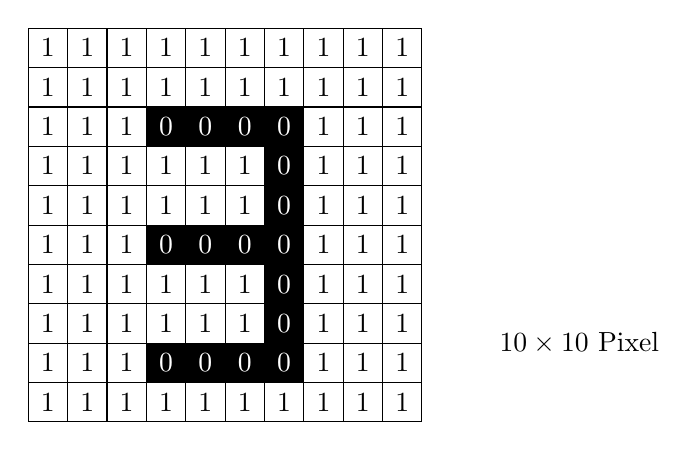
\begin{tikzpicture}
			
			%        \only<5->
			{
				\foreach \j in {0.5,1,...,5} 
				{
					\foreach \i in {0.5,1,...,5} {
						
						\node (P1) at (\i-0.25,\j-0.25) {1};
					}
				}
			}
			
			\draw[step=0.5,black,thin] (0,0) grid (5,5);
			
			%        \only<2->
			{
				
				\draw[fill=black] (1.5,0.5)  -- (2,0.5) -- (2,1) -- (1.5,1) -- cycle;
			}
			%        \only<3->
			{
				
				\draw[fill=black] (1.5,0.5)  -- (3.5,0.5) -- (3.5,1) -- (1.5,1) -- cycle;
				\draw[fill=black] (3,1)  -- (3.5,1) -- (3.5,4) -- (3,4) -- cycle;
				\draw[fill=black] (1.5,2)  -- (3.5,2) -- (3.5,2.5) -- (1.5,2.5) -- cycle;
				\draw[fill=black] (1.5,3.5)  -- (3.5,3.5) -- (3.5,4) -- (1.5,4) -- cycle;
			}
			
			%        \only<4->
			{
				\node (P1) at (1.75,0.75) {\textcolor{white}{0}};
				\node (P1) at (2.25,0.75) {\textcolor{white}{0}};
				\node (P1) at (2.75,0.75) {\textcolor{white}{0}};
				\node (P1) at (3.25,0.75) {\textcolor{white}{0}};
				\node (P1) at (3.25,1.25) {\textcolor{white}{0}};
				\node (P1) at (3.25,1.75) {\textcolor{white}{0}};
				\node (P1) at (3.25,2.25) {\textcolor{white}{0}};
				\node (P1) at (3.25,2.75) {\textcolor{white}{0}};
				\node (P1) at (3.25,3.25) {\textcolor{white}{0}};
				\node (P1) at (3.25,3.75) {\textcolor{white}{0}};
				
				\node (P1) at (1.75,2.25) {\textcolor{white}{0}};
				\node (P1) at (2.25,2.25) {\textcolor{white}{0}};
				\node (P1) at (2.75,2.25) {\textcolor{white}{0}};
				
				\node (P1) at (1.75,3.75) {\textcolor{white}{0}};
				\node (P1) at (2.25,3.75) {\textcolor{white}{0}};
				\node (P1) at (2.75,3.75) {\textcolor{white}{0}};
			}
			
			%        \only<6->
			{
				\node (Pixel) at (7,1) {$10 \times 10$ Pixel};
			}      
			
		\end{tikzpicture}
	\end{center}    
	
	
	\caption{Struktur eines Schwarz-Weiß-Bildes mit $10 \times 10$ Pixel}\label{img:schwarzweiss}
\end{figure}


Typische Auflösungen für Kamerabilder sind in der Tabelle\ref{Bild:Aufloesung} festgehalten. Ein Pixel ist durch die Anzahl der Farben und der Farbtiefe festgelegt. Die Farbtiefe gibt an, welchen Wertebereich die einzelnen Elemente entnommen sind. Dies sind in der Regel ganzzahlige Werte, der in Bit angegeben wird. So entspricht ein 8-Bit-Wert eine Zahl zwischen 0 und 255. Ein Pixel kann nun für jede Farbe einen solchen Zahlenwert enthalten. Häufig wird aber für jede Farbe eine eigene  Matrix verwendet. Falls man mit der RGB-Darstellung arbeitet, so hat man die Farben Rot, Grün und Blau. Durch Überlagerung der drei Bilder bei der Darstellung erhält man den Farbeindruck. Der Sachverhalt ist in der Abbildung~\ref{Bild:lenaRGB} dargestellt. 



\begin{table}
	\centering
	\begin{tabular}{lcc}
		Auflösung       &=& Breite $\times$ Höhe \\
		VGA             &=& $640 \times 480$ \\
		HD              &=& $1280 \times 720$\\
		Full HD         &=& $1920 \times 1080$\\
		4K              &=& $3840 \times 2160$\\
	\end{tabular}
	\caption{Standardauflösungen von Kamerabildern}\label{Bild:Aufloesung}  	
\end{table}

\bigskip



\begin{figure}
	\centering
	\begin{tikzpicture}
		\node (P1) at (0,0) {\includegraphics[width=0.2\textwidth]{Images/LenaBlue}};
		\node (P1) at (2,0) {$+$};
		\node (P1) at (4,0) {\includegraphics[width=0.2\textwidth]{Images/LenaRed}};
		\node (P1) at (6,0) {$+$};
		\node (P1) at (8,0) {\includegraphics[width=0.2\textwidth]{Images/LenaGreen}};
		\node (P1) at (10,0) {$=$};
		\node (P1) at (12,0) {\includegraphics[width=0.2\textwidth]{Images/lena}};
	\end{tikzpicture}
	\caption{Bild mit 3 Farbkanälen}\label{Bild:lenaRGB}
\end{figure}

Häufig werden statt Farbbild auch Graustufen verwendet. Hierzu werden häufig 256 Graustufen verwendet.% gemäß Abbildung~\ref{Bild:256Grustufen}. 
Bei der Umwandlung eines Farbbildes mit drei Farben werden die drei Matrizen gewichtet addiert. Es hat sich gezeigt, dass eine gleiche Gewichtung der Farbkanäle ungeeignet ist. Die Bibliothek OpenCV zur Bearbeitung von Bildern verwendet folgende Gewichtung \cite{OpenCV:2020b}:

% Quelle: https://latexref.xyz/_005cincludegraphics.html
$$0.299 \cdot \hbox{Red} +0.587 \cdot \hbox{Grün} +0.114 \cdot \hbox{Blau}$$

Die Umrechnung kann auf das Bild \glqq Lena \grqq{} angewendet; dies ist in der Abbildung~\ref{Bild:lenaGray}. Je nach Anwendung werden andere Gewichte verwendet. 
Obige Gewichte sind empirisch ermittelt und sind proportional zur
Empfindlichkeit des menschlichen Auges für jede der Trichromat-Farben. 
Das Bild~\ref{Bild:lenaGray} hat eine Farbtiefe von 8-Bit. Es können auch andere Farbtiefen verwendet werden. Ein Schwarz-Weiß-Bild hat die geringste Farbtiefe. 

\begin{figure}[!h]
	\begin{center}
		
		%\begin{subfigure}[h]{0.4\linewidth}
		%todo Eigene Bilder    
		\includegraphics[width=0.7\textwidth]{Images/graylena}
		
		\caption{Graustufen mit einem Wertebereich von 0 bis 255}\label{Bild:lenaGray}
	\end{center}    
\end{figure}




\begin{figure}[!h]
	\begin{center}
		
		%\begin{subfigure}[h]{0.4\linewidth}
		%todo Eigene Bilder    
		
		\includegraphics[width=0.3\textwidth]{Images/lenaBlackWhite126}
		\quad
		\includegraphics[width=0.3\textwidth]{Images/Grayscale4}
		\quad
		\includegraphics[width=0.3\textwidth]{Images/graylena}
		
		\caption{Schwarz-Weiß-Bild, Bild mit 4 Graustufen und mit 256 Graustufen.}\label{Bild:}
	\end{center}    
\end{figure}


Die Qualität der Bildes hängt aber nicht nur von den genannten Kenngrößen ab. Die Bildschärfe trägt auch dazu bei. Allerdings liegt hier leider keine einfache Definition vor, sondern wird häufig vom subjektiven Empfinden geprägt. Andererseits besteht die Möglichkeit, durch mathematische Operationen die Bildschärfe zu beeinflussen.  Unschärfe eines Bildes kann durch das Blurring erreicht werden. 
Jeder Pixelwert wird dabei durch den Durchschnitt der Pixelwerte in einem kleinen Fenster, das auf das Pixel zentriert ist. 

Die Auflösung des Bildes beeinflusst den Rechenaufwand. Für ein Bild mit einer
Auflösung von $674 \times 1200$ und einer Fenstergröße von $101 \times 101$ muss der neue Pixelwert für alle drei Farbkanäle separat berechnet werden. Insgesamt ergeben sich

$$674 \cdot 1200 \cdot 101 \cdot 101 \approx 8.2 \cdot 10^9$$

Operationen. Ein Beispiel ist in der Abbildung~\ref{Bild:Blurring} mit einer Filtergröße $5 \times 5$ dargestellt.


\begin{figure}
  \centering
  
  \includegraphics[width=0.3\textwidth]{Images/lenaBlurring}

  \caption{Weichgezeichnetes Bild mit einem $5 \times 5$-Filter}\label{Bild:Blurring}
\end{figure}


Eine andere Möglichkeit der Bildverarbeitung ist die Kantendetektion. Bei der Kantendetektion ist das Ziel, Regionen des Bildes zu identifizieren, wo Intensitäten der Farbe sich stark unterscheiden. Dies wird zum Abgrenzen von Objekten und zur
Objekterkennung verwendet. Ein Beispiel ist in Abbildung~\ref{Bild:Kanten} gegeben.

%
%Was ist ein Rand in einem Bild?
%Horizontaler Rand in Reihe i: Bild(i-1,j) unterscheidet sich stark
%von Bild(i+1,j)
%Vertikale Kante bei Spalte j: Bild(i,j-1) unterscheidet sich stark von
%Bild(i,j+1)
%Idee: Berechnen Sie für jede Position (i,j) und jede Farbe (RGB)
%change_hor = image(i-1,j, color) - image(i+1,j, color)
%change_vert = image(i,j-1, color) - image(i,j+1, color)
%edge_image(i,j,color) = sqrt( change_hor 2 + changevert 2 )
%

\begin{figure}
	\centering
	
	\includegraphics[width=0.3\textwidth]{Images/lenaBlackWhite}
	
	\caption{Kantendetection bei einem Bild}\label{Bild:Kanten}
\end{figure}

%    \includegraphics[width=0.7\textwidth]{Images/lena}
%    \includegraphics[width=0.7\textwidth]{Images/rgbChannel}


%todo https://gist.github.com/MarcWang/b8e715200775079e4653


%\begin{figure}
%  \centering
%  \begin{tikzpicture}
%     \draw[\fill=left color=black!100!black,right color=white]  rectangle(0.7*\paperwidth,7mm);
%                
%                %            \fill[path fading=south,black!60!white](0,0)rectangle(\paperwidth,-0.1cm);
%                %            \node[text=white,anchor=west,text width=0.7\paperwidth, inner sep=0pt] at (0.03\paperwidth,1.5) {};
%        
%        
%        \node (P1) at (0,1) {0};
%        \node (P2) at (10,1) {255};
%        
%  \end{tikzpicture}
%  \caption{Balken mit 256 Graustufen}\label{Bild:256Grustufen}
%\end{figure}    

